% \begin{preamble}
\documentclass[11pt]{article}
\usepackage[margin=1in]{geometry}
\usepackage[utf8]{inputenc}
\renewcommand{\rmdefault}{phv} % Arial Font
\renewcommand{\sfdefault}{phv} % Arial Font
\usepackage{color}
\usepackage{tcolorbox}
\usepackage{graphicx}
\usepackage{ragged2e}
\graphicspath{ {./figures/}} % Location of the graphics files
\usepackage[labelfont=bf]{caption}
\usepackage{multicol}
\usepackage{nopageno} % remove page numbers
\pagestyle{empty} % remove page numbers
\usepackage{gb4e}
\noautomath
% \end{preamble}

\newcommand{\glr}{\textcolor{teal}}
\definecolor{Purple}{RGB}{255,10,140}
\newcommand{\jd}[1]{\textcolor{Purple}{[jd: #1]}}
\newcommand{\mm}[1]{\textcolor{teal}{[mm: #1]}}


\begin{document}
% Title
\centerline{\textbf{Affect First? Evaluating the Affect First Hypothesis Through Valence}}
\centerline{Morgan Moyer, Anouch Bourmayan, Isidora Stojanovic and Brent Strickland}
% \centerline{mcmoyer11@gmail.com}%names
% Endtitle 

\noindent \textbf{Introduction}
If someone yelled ``Hey f*ck you!'', you would feel quite flummoxed and not a little emotional. \textbf{Valence} is a word's subjective affective meaning, positive/negative value. The expletive's negative valence is core to its meaning. Words also have a Conceptual meaning dimension: the verb `love' is generally positive, but also generally psychological/abstract. In contrast, `hug', while positive, is physical/concrete. The \textbf{Affect First Hypothesis} (AFH) [1,2] holds that affective information is processed before conceptual information, thus predicts word valence judgments are quicker than conceptual judgments. This seems clear for expletives/slurs, which trigger a physiological response (``hot'' affect). Does it hold for `love'/`hug' where judging them positive probably doesn't entail an elevated heart rate (``cold'' affect)? Across several experiments, we ask:

% If a long thin projectile is hurled at you, your instict likely is to duck, potentially in fear. 
% You probably felt your heart rate accelerate, your palms sweaty, and the sharp release of adrenaline that compelled you to action. 
% This emotion-first response occurs before you identify what the unidentified flying object is. 

\vspace{-.3cm}
\begin{tcolorbox}[colback=white]
\vspace{-.2cm}
\centering
\textbf{Q1 (specific)}: Are valence judgments cognitively prior to conceptual judgments? \\ 
\textbf{Q2 (broad)}: How should word valence be represented in the lexicon?
\vspace{-.2cm}
\end{tcolorbox}
\vspace{-.2cm}
\noindent \textbf{Background}
Since Frege, affective meaning is typically analyzed as not-strictly-truth-conditional, thus often sidelined with phenomena like slurs, expressivity, and evaluativity [3-9]. Affect helps hearers predict speaker meaning in slur processing [10], but support for AFH is mixed [11-15]. Task effects [15,16] and the communicative situation [17a] can both modulate affect effects. Identifying an adequate conceptual dimension for comparison that holds for most words is notoriously challenging [18a-21], so we pit Valence against multiple conceptual categories to answer Q1/Q2. We present pilot data that seem to support AFH and the central role of valence for word meaning.

% Stojanovic and Kaiser (2023) distinguish between true valenced adjectives and neutral adjectives

% Psycho- and neurolinguistic studies of the lexicon has looked at the valence properties of words in isolated contexts. 
% There is lots of evidence that valence interacts with many factors, including word category


\noindent \textbf{Exp1/2: Categorization tasks}. A binary-forced choice task where participants categorize single words as quickly as possible. We measure Reaction Time and Response (or Accuracy where unambiguous). \textbf{Exp1 (n=12)} stimuli use physical/psychological as Conceptual foil. 
% In a norming pretest (n=96), 7-point Likert ratings for both Valence (pos/neg) and Descriptive (physical/psychological) were taken for 168 verbs from [17]. 
40 verbs chosen from pretest norming represent the best of each combination of features (pos+phys, pos+psych, neg+phys, neg+psych) to reduce uncertainty about word categorization as a potential confound on Reaction Time. 
\textbf{Exp2 (n=20)} stimuli use concrete/abstract as Conceptual foil. 40 Verbs were selected via norming pretest from various sources, including [22,23].
\textbf{Results} Analyses used linear mixed effects models. RTs for Valence were faster than either Conceptual categorization ($t$=3.02, $p<$.003; Exp2: $\beta$=-0.168, $SE$=0.0389, $t$=-4,309, p$<$.0003). In Exp2, we find responses are less Accurate in the Concrete Task, and participants take longer to respond (\ref{fig:exp2-items}, $\beta$=0.151, $SE$=0.044, $t$=3.406, p$<$0.0007). Nonetheless, most verbs maintained faster RTs on Valence Task.

\noindent \textbf{Exp3: Similarity judgments (n=62)} are used to measure word meaning [24,25]. If Valence is central, then Valence-based similarity more than conceptual-based similarity would ground responses. Participants rated word similarity on a 7-pt scale. Word pairs were constructed by manipulating feature values from Exp1 words: Control Pairs match features %(SameVal+SameCon, DiffVal+DiffCon) 
Test Pairs mismatch. Participants responded based on Valence and not Conceptual similarity (Fig.~\ref{fig:exp3}, $t$=6.41, $p<$.0001). 



\noindent \textbf{Discussion}
Valence judgments are consistently faster than Conceptual judgments (Q1). While poor Accuracy did increase RTs for the Conceptual Task, most high accuracy words still maintained faster RTs on Valence Task. This is compelling evidence for AFH and the importance of affect for word meaning. Are there more basic linguistic categories than physical/psychological and abstract/concrete? We plan to further test AFH for cases where Conceptual judgments may be more clear (event vs. object, noun vs. verbs). Exp3 Results show hearers judge similarity on Valence more than Conceptual overlap, suggesting valence could be part of lexical meaning (Q2). Additionally, exploratory results suggest that valence judgments can vary depending on the surrounding words (during norming, particular Word List accounted for some effects %$\chi^2$(24)=232.2, 
$p<$.0001), compatible with effects of lexical alternatives. This tentative result resonates with contextual sensitivity of affect effects [15-17a], and probes the nature of context sensitivity in the lexicon.

% ghost lines to reserve space for author names
% \centerline{}

\newpage


\noindent
\begin{minipage}{0.5\linewidth}
\begin{tcolorbox}[colback=white]
    \hspace*{-.3cm}
    \vspace{-.5cm}
    % \centering
    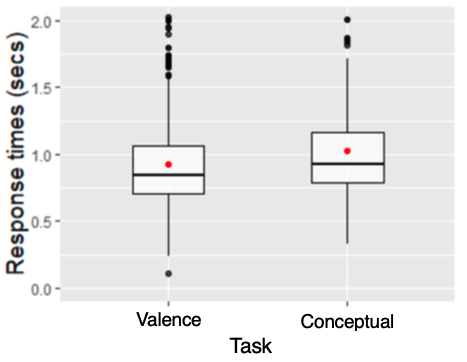
\includegraphics[scale=0.4]{figures/exp1.png}
    \vspace{.2cm}
    \centering
    \captionof{figure}{Exp1 Results: Faster RTs for Valence judgments than Conceptual categorization (physical vs. psychological).}
    \label{fig:exp1}
\end{tcolorbox}
\end{minipage}
\hfill
\begin{minipage}{0.48\linewidth}
    \begin{tcolorbox}[colback=white]
    \vspace{-.3cm}
    \centering
    % 
\includegraphics[scale=0.6]{figures/legend.png}
    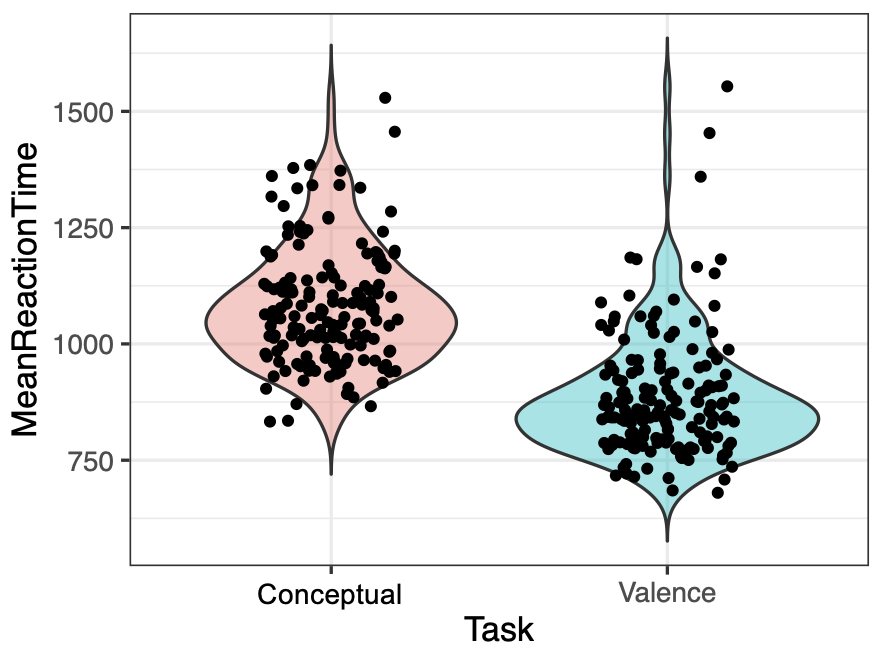
\includegraphics[scale=0.45]{figures/exp3.png}
    \vspace{-.75cm}
    \captionof{figure}{Exp2 Results: replication of Exp1 for concrete vs. abstract: $\beta$ = -0.168, $SE$ = 0.0389, $t$ = -4,309, $p$ $<$ .0003}

    \label{fig:exp2}
    \vspace{-.2cm}
    \end{tcolorbox}
\end{minipage}

\vspace{.2cm}

\noindent
\begin{tcolorbox}[colback=white]
\begin{minipage}{0.75\linewidth} 
    \vspace{-.3cm}
    % \hspace{-.5cm}
    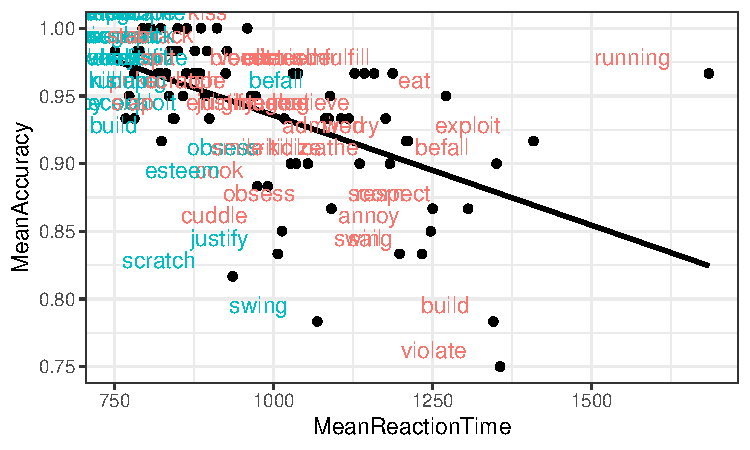
\includegraphics[scale=0.75]{figures/exp1b_accXrt.pdf}
    \vspace{-.2cm}
    % \hspace{1cm}
\end{minipage}
\hspace{-1.5cm}
\begin{minipage}{0.3\linewidth} 
\vspace{-.5cm}
    
\includegraphics[scale=0.5]{figures/legend.png}
    % \vspace{-.7cm}
    % \hrule
    % \vspace{.3cm}
    \captionof{figure}{From Exp2, TaskXAccuracy on RT: in Concrete task, responses less accurate and longer ($\beta$ = 0.151, $SE$ = 0.044, $t$ = 3.406, $p$ $<$ 0.0007). However, as accuracy in the Concrete Task increased, reaction time decreased.}
    \label{fig:exp2-items}
    \vspace{-.5cm}
\end{minipage}
\end{tcolorbox}

\begin{tcolorbox}[colback=white]
\begin{minipage}{0.5\linewidth}
    \vspace{-.2cm}
    % \hspace{-.5cm}
    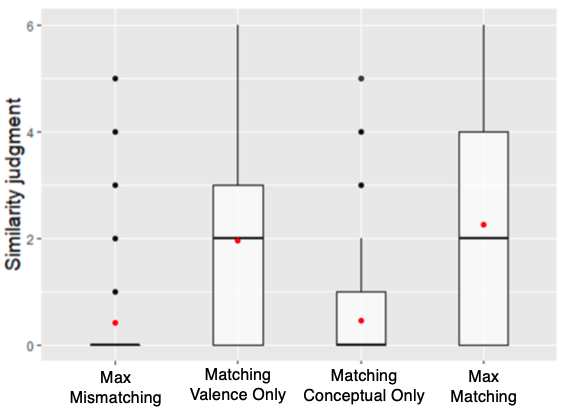
\includegraphics[scale=0.3]{figures/exp2.png}
    \vspace{-.2cm}
\end{minipage}
\begin{minipage}{0.45\linewidth}
    \captionof{figure}{Exp3 Results: Similarity judgment task, slider from 0 (dissimilar) to 6 (similar). Participants are more likely to rate verb similarity based on matching Valence (M = 1.97, SD = 1.73), than on matching Conceptual feature (physical/psychological) (M =.47, SD =.88).}
    \label{fig:exp3}
    % \vspace{-.5cm}
    % \hspace{1cm}
    
\end{minipage}
\end{tcolorbox}

\noindent \textbf{References}.
[1] Wundt 1907
[2] Zajonc 1980, 2000
[3] Potts 2005 
[4] Schlenker 2007 
[5] Kaplan 1999 
[6] McCready 2010 
[7] Gutzmann 2015 
[8] Stojanovic \& Kaiser 2023 
[9] Stojanovic in press 
[10] Ronderos \& Domaneschi 2023 
[11] Storbeck \& Robinson 2004 
[12] Storbeck \& Clore 2007 
[13] Nummenmaa, Hyönä \& Calvo 2011 
[14] Rohr \& Wentura 2023 
[15] Hinojosa, Moreno \& Ferré 2019 
[16] Hinojosa, Herbert, \& Kissler 2023
[17a] Rohr \& Abdel Rahman 2015 
[17] Levin 1993
[18] Kousta, Vigliocco, Vinson, Andrews and Del Campo 2011 
[18a] Lynott, Connell, Brysbaert, Brand \& Carney 2019 
[19] Vigliocco, Kousta, Della Rosa, Vinson, Tettamanti, Devlin, et al. 2014 
[20] Winter 2022 
[21] Herbert 2023 
[22] Warriner, Kuperman \& Brysbaert 2013,
[23] Brysbaert, Warriner \& Kuperman 2013
[24] Degen 2015 
[25] De Deyne, Perfors and Navarro 2016

\end{document}


